\documentclass[a4paper,11pt]{article}

% Use utf-8 encoding for foreign characters
\usepackage[utf8]{inputenc}
\usepackage[british,english]{babel}
\usepackage[T1]{fontenc}

% Setup for fullpage use
\usepackage{fullpage}

% Multipart figures
\usepackage{subfigure}

% More symbols
\usepackage{amsmath}
\usepackage{amssymb}
\usepackage{latexsym}

% For pretty URLs, see: http://en.wikibooks.org/wiki/LaTeX/Hyperlinks
\usepackage{hyperref}

% Surround parts of graphics with box
\usepackage{boxedminipage}

% Package for including code in the document
\usepackage{listings}

% If you want to generate a toc for each chapter (use with book)
\usepackage{minitoc}

% Uncomment if you want to use Palatino as font
\usepackage[sc]{mathpazo}
\linespread{1.05}         % Palatino needs more leading (space between lines)

% This is now the recommended way for checking for PDFLaTeX:
\usepackage{ifpdf}

%\newif\ifpdf
%\ifx\pdfoutput\undefined
%\pdffalse % we are not running PDFLaTeX
%\else
%\pdfoutput=1 % we are running PDFLaTeX
%\pdftrue
%\fi

\ifpdf
\usepackage[pdftex]{graphicx}
\else
\usepackage{graphicx}
\fi
\title{Deliverable 3: Sprint \#1\\\small{for}\\\small{Danske Bank: Peer-to-peer}}
\author{ Group Delta:\\Jesper Borgstrup, Thomas Kjeldsen and Mads Ohm Larsen }

\date{March 11, 2011}

\begin{document}

\ifpdf
\DeclareGraphicsExtensions{.pdf, .jpg, .tif}
\else
\DeclareGraphicsExtensions{.eps, .jpg}
\fi

\maketitle

%\tableofcontents
%\vspace{2cm}

\section{Requirements for this deliverable}
\begin{enumerate}
\item Doing a demo in class (on 2011-03-09)
\item Giving us access to your source code
\item Handing in a collection of your sprint material
\item Describing a sprint retrospective (e.g., as a set of bullets outlining what
when well, what went wrong, and how you will improve for the next sprint)
\end{enumerate}

The Sprint Demo was given on March 9th. This document describes requirements 2-4.

\section{Source code access}
Our source code is publicly available on Github from \url{https://github.com/omegahm/DBP2P}.

Please note that we are working on multiple branches (use the button switch branch to view another branch).

The master branch currently holds only documentation and deliverables, while we have a dedicated development branch for sprint \#1 named \texttt{dustytuba}.

If you wish to checkout our code (read-only) using Git, then use git clone with this URL:
\url{git://github.com/omegahm/DBP2P.git}


\section{Sprint material}
%TODO
Sprint Material needed to assess our progress include the following:
\begin{itemize}
\item source code (version number and access method is sufficient)
\item product backlog (before and after the sprint)
\item sprint backlog
\item any other material (e.g., burndown chart) that illustrates your progress
\end{itemize}

% TODO: Describe Acunote in general and that access have been granted.

\subsection{Source Code}

The final product of sprint \#1 has been merged into the master branch as per commit-id  \href{https://github.com/omegahm/DBP2P/commit/1abf2360b074729c7f2eefacb294f21fb668f9db}{1abf2360b074729c7f2eefacb294f21fb668f9db}.

The code and tests are located in the folders ``DustyTuba'' and ``DustyTuba''.

\subsection{Product Backlog}
The following tasks have been completed during this sprint:
\begin{itemize}
	\item Some Sprint \#0 stuff:
	\begin{itemize}
		\item Setup of git
		\item Setup of Acunote
	\end{itemize}
	\item Updated ``Product and Process Brief'' to fit new project
	\item Sample app
\end{itemize}

In regards to our user stories, the tasks completed corresponds to the following user stories:
\begin{verbatim}
  As a        user
  I want to   identify a nearby device
  Such that   I can establish a connection in order to transfer information safely	

  As a        user
  I want to   identify a nearby device using Bump
  Such that   I can establish a connection in order to transfer information safely
\end{verbatim}

\subsection{Sprint Backlog}
Our sprint backlog is shown in figure \ref{sprintbacklog} on page \pageref{sprintbacklog}.
As seen we have a ``Not started'' task. 
This task will be moved to sprint \#2.

\begin{figure}[ht!]
	\begin{center}
	% Insert sprint backlog here
	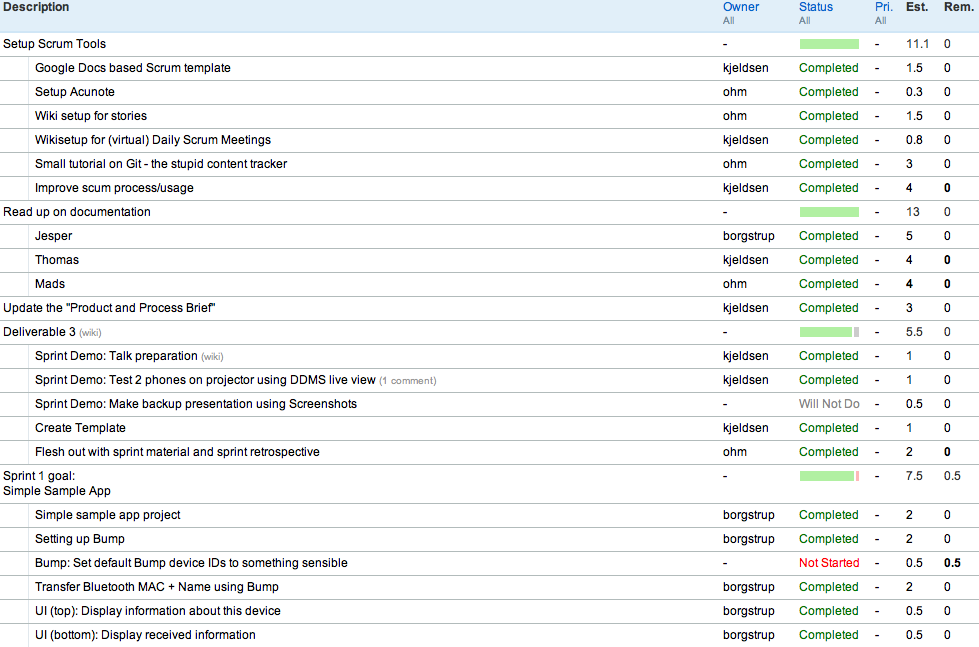
\includegraphics[width=1.4\textwidth, angle=-90]{sprintbacklog.png}		
	\end{center}
	\caption{Our sprint backlog after the sprint was finished}
	\label{sprintbacklog}
\end{figure}

\subsection{Burndown chart}

Our burndown chart is shown in figure \ref{burndown} on page \pageref{burndown}.
The reason for the steep descends is that we changed from Google Docs during the sprint.
The ``Not assigned'' line moves into our individual line when a job is assigned, and does not reflect that a job of one hour have been not assigned for the entire course of sprint \#1.

\begin{figure}[ht!]
	\begin{center}
	% Insert burndown chart here
	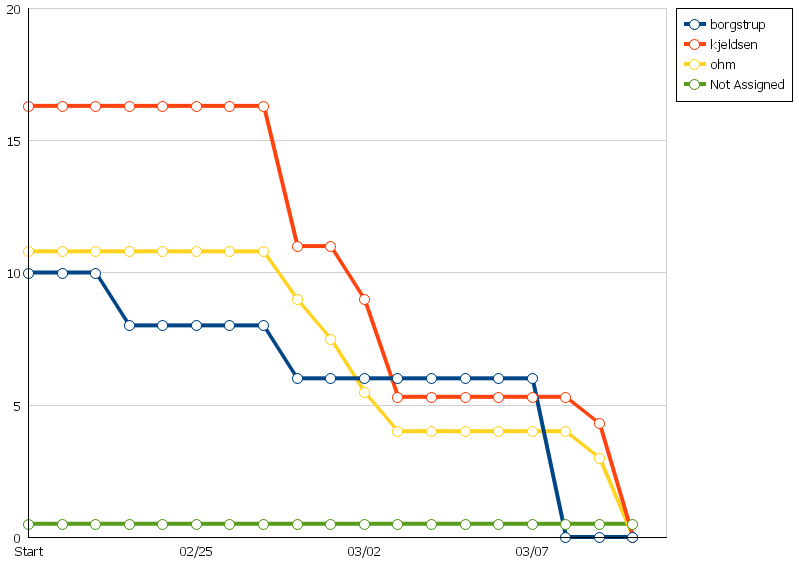
\includegraphics[width=\textwidth]{burndown.png}		
	\end{center}
	\caption{Our burndown chart at the end of the sprint}
	\label{burndown}
\end{figure}

\subsection{Other relevant material}
We have got an Acunote account\footnote{\url{http://dbp2p.acunote.com/}} setup, and access to this have been granted.

\clearpage
\section{Sprint retrospective}

What went well during this sprint:

\begin{itemize}
	\item We held scrum meetings via Skype, which allows us to refer back to our chat-logs later
	\item We setup a shared calender, which updates automatically
	\item Migration to Acunote to track our scrum process
	\item We reimagined the scope of our project and delivered what we set out to do
	\item Honesty between team members
\end{itemize}

\noindent
What went wrong:

\begin{itemize}
	\item We need to be better to communicate. Despite our shared calender, we had some hick-ups in meeting times
	\item We did not explicitly enough state ahead of time who held the role of scrum master
	\item Distribution of code workload among team members, rested primarily on one member 
	\item Lack of breakdown of sprint goals in the beginning of the sprint
	\item Failure to understand Git 
	\item Chat meetings were useful, but they sometimes went idle until someone pushed the issue
\end{itemize}

\noindent
How we will improve:
\begin{itemize}
	\item We'll choose our scrum master, and this person has the scrum master responsibilities from day one
	\item We’ll plan ahead and clearly state when, where and how we’re going to meet (chat, voice chat, physical meeting)
	\item We’ll do actual “daily scrum” meetings whenever we meet physically
	\item We’ll breakdown stories into tasks, clearly define the sprint backlog, estimates and assign workload prior to starting the sprint
	\item We'll read up on the Git configuration management\footnote{\url{http://excess.org/article/2008/07/ogre-git-tutorial/}}
\end{itemize}

\end{document}
